\chapter{Revisão Bibliográfica}

A pesquisa bilbliográfica deste trabalho é delineada pelo estudo de sistemas
multicorpos, que faz uma revisão da modelagem cinemática e dinâmica desses
sistemas; a análise dinâmica de estruturas, que busca métodos para obter a
matriz de rigidez e amortecimento da base; a pesquisa sobre manipuladores
robóticos compostos por elementos flexíveis; e tarefas robóticas de precisão
\textit{in situ}.


% -.~.-.~.-.~.-.~.-.~.-.~.-.~.-.~.-.~.-.~.-.~.-
\section{Dinâmica de Sistemas Multicorpos}

A dinâmica de sistemas multicorpos (MBS) é baseada na mecânica clássica. Esses
sistemas são definidos por um ou mais corpos, imperfeitamente conectados, pela
possibilidade de movimento relativo entre eles. A conexão imperfeita de 2 ou
mais corpos rígidos que forma o sistema multicorpo é denominado par cinemático,
ou junta~\cite{de2012kinematic}. Dinâmica multicorpos pode ser entendida como o
estudo de sistemas de vários corpos sujeitos a forças e interações devido a
diferentes tipos de juntas que os conectam e restringem seu
movimento~\cite{flores2008kinematics}, como ilustrado esquematicamente na
Figura~\ref{fig::mbs_diagram}.

\begin{figure}[h]
	\centering 
 	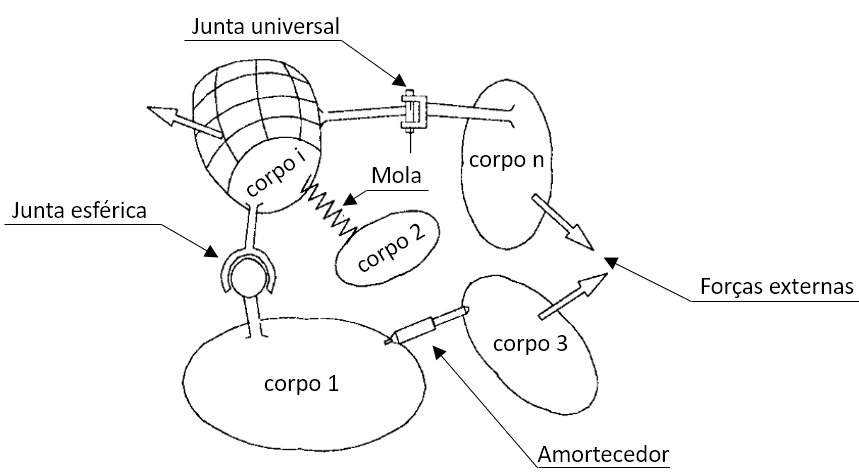
\includegraphics[width=0.75\textwidth]{figs/mbs_diagram}
 	\caption[Representação de um sistema MBS]{Representação de um sistema MBS.
 	\\Fonte: adaptado de \cite{neto2003stabilization}}
 	\label{fig::mbs_diagram}
\end{figure}

A mecânica clássica dos sistemas de corpos rígidos e suas aplicações foram
marcadas por fortes restrições na complexidade dos modelos até a década de 1960.
Entretanto, a necessidade de modelar sistemas mais complexos, como satélites e
veículos espaciais, assim como a rápida evolução dos computadores na época,
abriram caminhos para aplicações mais avançadas de sistemas
multicorpos~\cite{schiehlen1997multibody}.

Hoje, muitos programas estão disponíveis para a modelagem e simulação de
sistemas MBS, e possuem interface gráfica e ferramentas para modelagem ou
importação de corpos CAD e elementos padronizados de conectores, como juntas de
de vários tipos, molas e amortecedores. Para citar alguns:
%
\begin{enumerate*}[label=\roman*]
	\item MSC ADAMS;
	\item Universal Mechanism;
	\item MapleSim.
\end{enumerate*}
%

No entanto, para ter maior controle da modelagem matemática, dos métodos e das
simplificações e tratamento e pós-processamento dos resultados, este trabalho
não fez uso de um programa comercial dedicado. Para isso, derivou-se toda a
cinemática, dinâmica e equações de movimento dos sistemas simbolicamente, no
Sophia-Maple. Isto permite que o método seja livre de restrições impostas pelas
capacidade de qualquer programa, tornando explícita a metodologia proposta e
permitindo repeti-la e verifica-la em qualquer outra plataforma.

Os fundamentos da cinemática e da dinâmica, tratados a seguir, são reunidos de
livros-texto de referência nas disciplinas de Dinâmica de Corpos Rígidos
\cite{tenenbaum2006fundamentals} e \cite{kane1985dynamics}, Sistemas Multicorpos
\cite{shabana2013dynamics} e Robótica \cite{sciavicco2012modelling} e
\cite{spong2006robot}. Esses autores guiam os conceitos básicos utilizados para
modelagem matemática dos sistemas multicorpos aqui apresentados.


\subsection{Cinemática}\label{sec::cinematica}

Na análise cinemática de sistemas multicorpos, apenas os aspectos geométricos
são estudados para descrever as posições, velocidades e acelerações dos corpos.
As forças e momentos que causam o movimento do sistema são considerados na
análise dinâmica.

\subsubsection{Sistemas de Coordenadas}

Um corpo rígido é completamente descrito por sua posição e orientação com
respeito a um sistema de coordenadas (SC). Um sistema de coordenadas é um
conjunto de eixos ortogonais que se inteceptam em um ponto, denominado origem.

Geralmente, em sistemas multicorpos, 2 tipos de SC são utilizados. O primeiro é
fixo no tempo e representa uma referência para todos os corpos, denominado
sistema de referência \emph{global} ou \emph{inercial}. O segundo tipo é
solidário a cada componente do sistema, representando um SC \emph{local}, que
translada e gira com o corpo.

A Figura~\ref{fig::sist_refs} apresenta um corpo B, seu referencial local SC-B e
um referncial inercial SC-R, que descrevem o mesmo ponto $p$ em B, por 2 vetores
diferentes.

\begin{figure}[h]
	\centering 
 	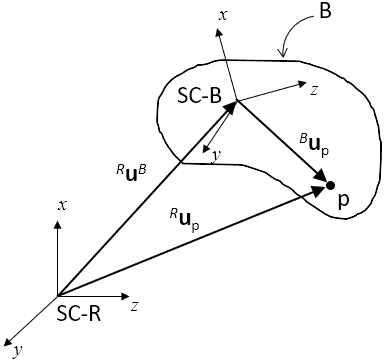
\includegraphics[width=0.45\textwidth]{figs/sist_refs}
 	\caption{Sistemas de referência global e local}
 	\label{fig::sist_refs}
\end{figure}

Os vetores que descrevem a posição do ponto $p$ em cada referencial podem ser
definidos com 3 coordenadas:
%
\begin{align}
	^{R}\textrm{\textbf{u}}^{p} = [r1, r2, r3]^{R} \\
	^{B}\textrm{\textbf{u}}^{p} = [b1, b2, b3]^{B}
\end{align}
%
Note-se que $^{R}\textrm{\textbf{u}}^{p}$ também pode ser escrito como a soma de
2 vetores:
%
\begin{equation}
	^{R}\textrm{\textbf{u}}^{p} = {}^{R}\textrm{\textbf{u}}^{B} + 
	{}^{B}\textrm{\textbf{u}}^{p}
\end{equation}
%

Logo, qualquer ponto no do corpo B pode ser descrito como uma soma da posição do
referencial do corpo, com respeito ao referencial global e o vetor posição do
ponto com respeito ao refencial local.


\subsubsection{Coordenadas generalizadas}

A configuração de um sistemas multicorpos é identificada por um conjunto de
variáveis chamadas \emph{coordenadas generalizadas}, que definem completamente a
posição e orientação de cada corpo no sistema.

Então, um corpo rígido no espaço pode ser descrito usando 6 coordenadas
independentes, 3 para posição da origem do corpo e 3 para orientação do corpo
com respeito ao referencial inercial. Estes parâmetros serão função das
coordenadas generalizadas.

As coordenadas generalizadas são usualmente simbolizadas pela letra
$q$, e numeradas de $1$ a $n$. Podem ser denotadas pelo seguinte vetor:
%
\begin{equation}
	\mathbf{q} = [q1, q2, q3,\ldots, qn]
\end{equation}
%
A variação das coordenadas generalizadas, ou seja, sua derivada no tempo, é
usualmente representada pela letra $u$. Logo:
%
\begin{equation}
	\frac{\mathrm{d} \mathbf{q}}{\mathrm{d} t} = \left[ \frac{\mathrm{d}
q1}{\mathrm{d} t}, ..., \frac{\mathrm{d} qn}{\mathrm{d} t}\right] \rightarrow  \mathbf{u} = [u1,...,un]
\end{equation}
%



% A escolha dos SC's impacta substancialmente no tamanho das equações
% cinemáticas que descrevem os movimentos dos corpos. Uma escolha perspicaz do conjunto de
% SC's utilizado é importante para a eficiência do código e do cálculo
% computacional.

\subsubsection{Matrizes de Rotação}

As matrizes de rotação definem a orientação relativa entre 2 sistemas de
coordenadas. As matrizes que representam as rotações básicas em torno
dos eixos $x, y$ e $z$ são: 
%
\begin{equation}
	R_{x,\theta} = 
\begin{pmatrix}
1 &0  &0 \\ 
0 &\cos(\theta)  &-\sin(\theta) \\ 
0 &\sin(\theta)  &\cos(\theta) 
\end{pmatrix}
\end{equation}
%
\begin{equation}
R_{y,\theta} = 
\begin{pmatrix}
\cos(\theta) &0  &\sin(\theta) \\ 
0 &1  &0 \\ 
-\sin(\theta) &0  &\cos(\theta) 
\end{pmatrix}
\end{equation}
%
\begin{equation}
R_{z,\theta} = 
\begin{pmatrix}
\cos(\theta) &-\sin(\theta)  &0 \\ 
\sin(\theta) &\cos(\theta)  &0 \\ 
0 &0  &1
\end{pmatrix}
\end{equation}
%

Uma matriz rotação geral $R$, pode ser definida pela sequência ilimitada de
quaisquer rotações básicas. Por exemplo:
%
\begin{equation}
	R_{ZYZ} = R_{z,\phi} \cdot R_{y,\theta} \cdot R_{z,\psi}
\end{equation}
%
Esta em especial representa um método comum para para especificar a matriz de
rotação que orienta um corpo em função 3 quantidades independentes $\phi,
\theta, \psi$, denominado \emph{Ângulos de Euler}, tal que de 3 rotações, não
ocorram 2 rotações sucessivas em torno do mesmo eixo.
Outros métodos comuns para especificar uma matriz de rotação são ângulos
\textit{Roll-Pitch-Yaw}, Quaternions~\cite{sciavicco2012modelling} e ângulos de
Bryan~\cite{wittenburg2013dynamics}.

Também é possível uma representação exponencial da matriz de rotação. É
demonstrado em~\cite{murray1994mathematical}, utilizando o método dos parâmetros
de Rodrigues, como representar a rotação $R \in \mathbb{R}^{3\times3}$, na forma
exponencial em termos de eixo, $\boldsymbol{\omega} \in \mathbb{R}^{3}$, e um
ângulo, $\theta \in \mathbb{R}$.
%
\begin{equation}
	R(\omega, \theta) = e^{\hat{\omega} \theta}
\end{equation}
%

Realizando o devido desenvolvimento matemático é possível chegar-se a uma
solução fechada para o ângulo e eixo correspondentes a uma matriz de rotação, de acordo com as
equações:
%
\begin{gather}
%eq1
	\theta =  \cos^{-1}\left(\frac{tr(R) - 1}{2}\right) \label{eq::ang_erro} \\
%eq2	
	\omega = \frac{1}{2 s_\theta} \begin{bmatrix}
r_{32}-r_{23}\\ 
r_{13}-r_{31}\\ 
r_{21}-r_{12}
\end{bmatrix} \label{eq::eixo_erro}
\end{gather}
%
Onde $r_{ij}$ são os componentes da matriz de rotação $R$ e $tr(R)$ o seu
traço.

As equações~\ref{eq::ang_erro} e \ref{eq::eixo_erro} são interessantes para o
método proposto neste trabalho por fornecer uma forma de calcular os erros de
orientação do efetuador do robô devido aos deslocamentos da base. É uma forma
mais conveniente e ilustrativa do que a representação matricial.



\subsubsection{Transformação Homogênea}

Se os referenciais são coincidentes, a representação de um vetor com respeito a
outro referencial é simplesmente a projeção do vetor através da matriz de
rotação:
%
\begin{equation}
^{A}\textrm{\textbf{p}} = R_{B}^{A} \cdot {}^{B}\textrm{\textbf{p}}
\end{equation}
%

Se um referencial fixo num corpo desloca-se em relação a outro referencial, como
na Figura~\ref{fig::sist_refs}, a representação de $p$ descrito em SC-R, poderia
ser escrita como:
%
\begin{equation} \label{eq::upemr}
	^{R}\textrm{\textbf{u}}^{p} = {}^{R}\textrm{\textbf{u}}^{B} + R \cdot
	{}^{B}\textrm{\textbf{u}}^{p}
\end{equation}
%

Uma forma mais prática de representar o deslocamento geral dos corpos do sistema
(rotação e translação) ao longo de diferentes referenciais é utilizando o
conceito de matrizes de Transformação Homogênea. É basicamente uma representação
do movimento rígido na forma matricial. 
\begin{equation}
	H = 
\begin{pmatrix}
R & d\\ 
0 & 1
\end{pmatrix} ~,~ \in ~ \mathbb{R}^{4\times4}
\end{equation}
%
Onde $R \in \mathbb{R}^{3\times3}$ representa a matriz de rotação e $d \in
\mathbb{R}^{3}$ o vetor translação entre os referenciais.

Logo, a equação~\ref{eq::upemr}, poderia ser representada simplesmente por:
%
\begin{equation}
	^R\bar{\mathbf{u}}^p = H_B^R \cdot {^B}\bar{\mathbf{u}}^p
\end{equation}
%
Onde:
%
\begin{equation}
	^R\bar{\mathbf{u}}^p = \begin{pmatrix}
^R\mathbf{u}^p\\ 
1
\end{pmatrix}
=
\begin{pmatrix}
R_B^R & {^R}\mathbf{u}^B\\ 
0 & 1
\end{pmatrix}
\begin{pmatrix}
^B\mathbf{u}^{p}\\ 
1
\end{pmatrix} =: H_B^R \cdot {^B}\bar{\mathbf{u}}^{p}
\end{equation}


\subsubsection{Velocidade Angular, Linear e Aceleração}

Assumindo que um referencial associado a um corpo C se move em relação
um referencial R, então há um vetor $^{R}\boldsymbol{\omega}^{C}$ tal que para
todo vetor $\mathbf{v}$ fixo em $C$, sua derivada temporal em relação ao
referencial $R$ é:
%
\begin{equation}
	\frac{\mathrm{d} \mathbf{v}}{\mathrm{d} t} = {}^{R}\boldsymbol{\omega}^{C}
	\times \mathbf{v}
\end{equation}
%
Onde ${}^{R}\boldsymbol{\omega}^{C}$ é chamado vetor velocidade angular
de C em R.
De uma forma mais geral, a relação de um vetor $\mathbf{u}$, com respeito a 2
referenciais, movendo-se arbitrariamente em relação um ao outro é expresso como:
%
\begin{equation} \label{eq::velgeral}
	\frac{^{A}\mathrm{d} \mathbf{u}}{\mathrm{d} t} = \frac{^{B}\mathrm{d}
	\mathbf{u}}{\mathrm{d} t} + {}^{A}\boldsymbol{\omega}^{B} \times \mathbf{u}
\end{equation}
%
A equação~\ref{eq::velgeral} define a velocidade do vetor $\mathbf{u}$ com
respeito ao referencial A. Portanto, do sistema genérico da
Figura~\ref{fig::sist_refs}, pode-se escrever a velocidade do ponto $p$ como:
%
\begin{equation}
	^{R}\mathbf{v}^{p} = {}^{B}\mathbf{v}^{p} + ^{R}\mathbf{v}^{B} +
	{}^{A}\boldsymbol{\omega}^{B} \times {}^{B}\textrm{\textbf{u}}^{p}
\end{equation}
%

A aceleração do ponto $p$ com respeito ao referencial R será a derivada temporal
da velocidade com respeito a R. Logo:
%
\begin{equation}
	^{R}\mathbf{a}^{p} = \frac{^{A}\mathrm{d} }{\mathrm{d} x} {^{R}\mathbf{v}^{p}}
\end{equation}
%
Fazendo-se a derivada temporal, obtém-se a expressão:
%
\begin{equation}
	^{R}\mathbf{a}^{p} = {}^{B}\mathbf{a}^{p} + {}^{R}\mathbf{a}^{B} +
	{}^{R}\boldsymbol{\omega}^{B} \times ({}^{R}\boldsymbol{\omega}^{B} \times
	{}^{B}\mathbf{u}^{p}) + {}^{R}\boldsymbol{\alpha}^{B} \times {}^{B}\mathbf{u}^{p}
	+ 2{}^{R}\boldsymbol{\omega}^{B} \times {}^{B}\mathbf{v}^{p}
\end{equation}
%
Onde ${}^{R}\boldsymbol{\alpha}^{B}$ é o vetor aceleração angular do referencial
B em relação a R e o termo $2{}^{R}\boldsymbol{\omega}^{B} \times
{}^{B}\mathbf{v}^{p}$ é o chamado \emph{aceleração de Coriolis}. 


\subsubsection{Cinemática de Manipuladores Robóticos}

Manipuladores robóticos consistem em um sistema mecânico composto por uma série
de corpos (elos), conectados por juntas. Cada junta fornece um, e apenas um,
grau de liberdade, podendo ser translacional (primsático) ou rotacional (juntas de
revolução). A estrutura de juntas de um robô pode ser descrita por uma sequência
de caracteres representando os tipos de juntas: ``R'' para rotacional e ``P''
para prismática. Logo, o manipulador MOTOMAN MH12 pode ser caracterizado por
RRRRRR, por exemplo, por ser formado por 6 juntas de revolução.

A formulação das relações cinemáticas permitem o estudo de um problema chave em
robótica, da cinemática direta, que consiste na determinação de um método
sistemático e geral para descrever a pose (posição e orientação) do
efetuador, $\xi_{E}$, em função do valor das juntas, $\mathbf{q}$. Pode ser
expresso matematicamente como:
%
\begin{equation}
	\xi_{E} = \mathcal{K}(\mathbf{q})
\end{equation}
%

Um método, presente em praticamente todos os livros de introdução a robótica,
utilizado para sistematização da análise cinemática de manipuladores robóticos,
é de \emph{Denavit-Hartenberg} (DH)~\cite{denavit1955}.
Consiste em uma convenção para fornecer sistematicamente as matrizes de
transformação homogênea de cada sistema de coordenadas a partir de apenas 4
parâmetros:
$a_i, \alpha_i, d_i, \vartheta_i$, que são respectivamente para cada elo $i$
comprimento, torção e \textit{offset} e o ângulo da junta.
Uma ilustração da utilização do método é apresentada na
Figura~\ref{fig::tipica_dh}, que representa um manipulador tipo pulso esférico
de 3 gdl e na Tabela~\ref{tab::param_dh} a estrutura típica de representação dos
parâmetros DH.

\begin{figure}[h]
	\centering 
 	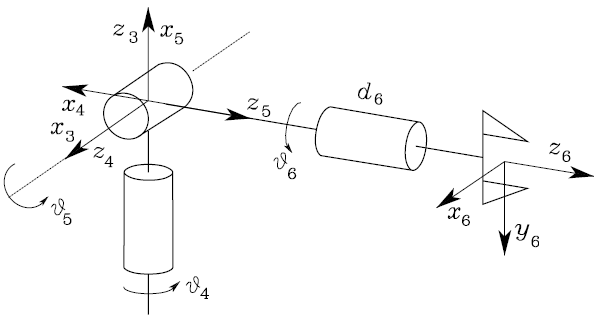
\includegraphics[width=0.55\textwidth]{figs/tipica_dh}
 	\caption[Manipulador tipo pulso esférico na convenção DH]
 	{Manipulador tipo pulso esférico na convenção DH \\
 	Fonte: adaptado	de~\cite{sciavicco2012modelling}}
 	\label{fig::tipica_dh}
\end{figure}

%
\begin{table}
\centering
\caption{Parâmetros DH do pulso esférico}
\label{tab::param_dh}
\begin{tabular}{@{}ccccc@{}}
\toprule
Elo & $a_i$ & $\alpha_i$ & $d_i$ & $\vartheta_i$ \\ \midrule
1   & 0     & $-\pi/2$   & 0     & $\vartheta_1$ \\
2   & 0     & $\pi/2$    & 0     & $\vartheta_2$ \\
3   & 0     & 0          & $d_6$ & $\vartheta_3$ \\ \bottomrule
\end{tabular}
\end{table}
%

\subsection{Cinemática Inversa}\label{sec::ikin}

O problema inverso, ou seja, encontrar o valor das juntas $\mathbf{q}$ que
satisfazem $\xi_{E}$, é feito pela análise da cinemática inversa. Logo:
%
\begin{equation} \label{eq::invq}
	\mathbf{q} = \mathcal{K}^{-1}(\xi_{E})
\end{equation}
%

A solução deste problema é de fundamental importância, porque transforma o
movimento desejado do efetuador, no espaço cartesiano, no valor correspondente
das juntas. Entretanto, o problema da cinemática inversa é muito mais complexo,
pelos seguintes motivos~\cite{sciavicco2012modelling}:
%
\begin{itemize}
  \item As equações a serem resolvidas são geralmente não lineares, então nem
  sempre é possível obter uma solução de forma fechada;
  \item Múltiplas ou infitas soluções podem existir;
  \item Dependendo da estrutura cinemática do manipulador, pode não existir
  solução admissível.
\end{itemize}
%

De qualquer forma, para o manipulador de 6 gdl modelo MOTOMAN MH12 que é tratado
nesta pesquisa, há pelo menos 16 soluções admissíveis. Este número é
reduzido quando considerados os limites de ângulo das juntas.

Os manipuladores comerciais evoluiram mantendo uma estrutura cinematicamente
simples, muito em virtude da dificuldade da solução da cinemática inversa.
Há hoje diversas
técnicas para resolver o problema inverso, o que tem permitido explorar
manipuladores mais complexos. Para citar alguns exemplos:
método geométrico~\cite{spong2006robot}, 
subproblemas de Paden-Kahan~\cite{murray1994mathematical}, 
Jacobiano Transposto, Pseudoinversa e Mínimos Quadrados
Amortecido~\cite{buss2004introduction}.

O método escolhido para resolver a cinemática inversa foi o geométrico, devido à
sua simplicidade e ao manipulador MH12 possuir uma estrutura cinemática bastante
favorável à solução por este método. É demonstrado a seguir a metodologia
apresentada por \citet{spong2006robot}, utilizando o conceito de desacoplamento
cinemático, para chegar à solução da equação~\ref{eq::invq} pela abordagem
geométrica.


\subsubsection{Desacoplamento cinemático}

Para manipuladores que possuem 6 juntas, tal que as 3 últimas se interceptam no
mesmo ponto, é posível desacoplar a cinemática inversa em dois subproblemas mais
simples: cinemática inversa de posição e cinemática inversa de orientação. Ou
seja, para manipuladores de 6 gdl com pulso esférico, o problema torna-se
simplesmente encontrar a posição da interseção das 3 últimas juntas e a
orientação do pulso. Este conceito será utilizado para modelagem da cinemática
inversa do robô MOTOMAN MH12.

A Figura~\ref{fig::decoupling} ilustra o conceito de desacoplamento, onde
$\mathbf{p}_W$ refere-se a posição da origem do pulso esférico, $\mathbf{p}_E$ a
posição do efetuador e $\mathbf{d}_E$ a distância do efetuador para o pulso na direção
de orientada pelo efetuador.

\begin{figure}[h]
	\centering 
 	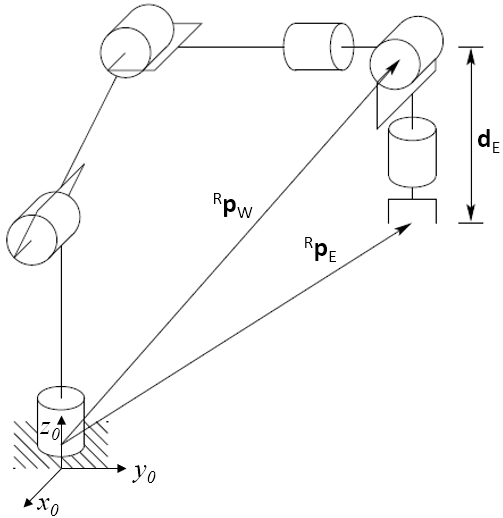
\includegraphics[width=0.45\textwidth]{figs/decoupling}
 	\caption[Desacoplamento cinemático]{Desacoplamento cinemático \\ Fonte:
 	adaptado de~\cite{spong2006robot}}
 	\label{fig::decoupling}
\end{figure}

Logo, pode-se definir a posição e orientação final da ferramenta acoplada ao
efetuador como:
%
\begin{equation}
	\mathbf{x}_{f} = \begin{bmatrix}
		\mathbf{p}_{f} \\ \boldsymbol{\Phi}_{f}
	\end{bmatrix}
	\label{eq::posf}	
\end{equation}
%
Onde $\mathbf{p}_{f}$ é um vetor das coordenadas da extremidade da ferramenta e
$\boldsymbol{\Phi}_{f}$ um vetor composto pelos ângulos de Euler que definem a
orientação da ferramenta.
%
\begin{align}
\mathbf{p}_{f} &= [x_f,y_f,z_f] \\
\boldsymbol{\Phi}_{f} &= [\phi,\theta,\psi]
\end{align}
%
Entretanto, a posição da ferramenta depende da posição do pulso, da orientação
e da distância entre o pulso e a ferramenta no referencial do pulso:
% 
\begin{equation} \label{eq::posfbib}
	\mathbf{p}_{f} = \mathbf{p}_{w} + [d_{x}, d_{y}, d_{z}]
\end{equation}
%
Logo, a solução da cinemática inversa, para o posição e orientação do pulso,
fornece a posição final da ferramenta, dada pela equação~\ref{eq::posfbib}.


\subsubsection{Solução da cinemática inversa de posicionamento}

Considerando-se apenas as 3 primeiras juntas do manipulador da
Figura~\ref{fig::decoupling}, e com auxílio das Figuras~\ref{fig::geom_pos_sup}
e \ref{fig::geom_pos_lat}, verifica-se as seguintes relações:
%
\begin{align}
	\theta_{1} &= \atantwo(x_c, y_c) \pm \atantwo(-\sqrt{r^2-d^2}, -d)
	\label{eq::theta1}\\
	\theta_{2} &= \atantwo(\sqrt{x_c^2+y_c^2-d^2}, z_c-d_1) - \atantwo(a_2+a_3
	c_3,a_3 s_3) \\
	\theta_{3} &= \atantwo(D, \pm \sqrt{1-D^2}) \label{eq::theta3}
\end{align}
%
Onde:
\begin{equation*}
		D = \frac{x_c^2+y_c^2-d^2 + (z_c-d_1)^2 - a_2^2 - a_3^2}{2a_2 a_3}
\end{equation*}
%
Os termos $x_c, y_c, z_c$ são a posição da extremidade do manipulador em que
é acoplado o pulso, $d$ é a distância de \textit{offset} da primeira junta,
$a_2$ e $a_3$ são os comprimentos dos elos. Utiliza-se a notação simplificada
das funções trigonométricas, portanto $s_2, c_2$, por exemplo, correpondem a
$\sin(\theta_2)$ e $\cos(\theta_2)$ respectivamente, o que valerá para todo o
texto.


\begin{figure}[h]
	\centering 
 	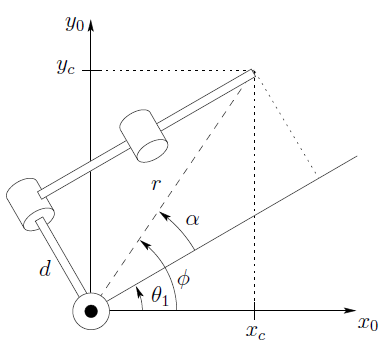
\includegraphics[width=0.45\textwidth]{figs/geom_pos_sup}
 	\caption[Vista na projeção xy do manipulador]{Vista na projeção xy do manipulador
 	\\ Fonte: adaptado de~\cite{spong2006robot}}
 	\label{fig::geom_pos_sup}
\end{figure}

\begin{figure}[h]
	\centering 
 	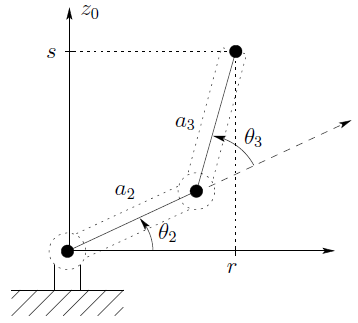
\includegraphics[width=0.45\textwidth]{figs/geom_pos_lat}
 	\caption[Vista na projeção xz do manipulador]{Vista na projeção xz do
 	manipulador \\ Fonte: adaptado de~\cite{spong2006robot}}
 	\label{fig::geom_pos_lat}
\end{figure}

Note-se que as equações encontradas fornecem 4 soluções de configuração do
manipulador para um mesmo ponto no espaço.

\subsubsection{Solução da cinemática inversa de orientação}

O problema da orientação inversa corresponde a encontrar os valores das 3 jnutas
do pulso para determinar a orientação desejada. A orientação desejada pode ser
definida pelos ângulos de Euler $\phi, \theta, \psi$ que transformam a
orientação do referencial inercial para a orientação final do referencial do
efetuador.
Então, basta encontrar os ângulos $\theta_4, \theta_5, \theta_6$ que satisfazem
a orientação desejada.

Logo, a equação que deve ser resolvida é a seguinte:
%
\begin{equation}
	R_3^6 = (R_0^3)^T R
\end{equation}


Pela matriz $R$ define-se a orientação final que se deseja alcançar pelo
efetuador.
Utilizando os ângulos de Euler para rotações em torno dos eixos ZYZ , fornece-se
a matriz que representa a orientação desejada:
%
\begin{equation} \label{eq::rzyz}
R_{zyz} = 
\begin{pmatrix}
c_\phi c_\theta c_\psi - s_\phi s_\psi & -c_\phi c_\theta s_\psi - s_\phi c_\psi & c_\phi s_\theta\\ 
s_\phi c_\theta c_\psi + c_\phi s_\psi & -s_\phi c_\theta s_\psi + c_\phi c_\psi & s_\phi s_\theta\\ 
-s_\theta c_\psi & s_\theta s_\psi & c_\theta
\end{pmatrix}
\end{equation}
%

A matriz transposta da rotação que leva do referencial inercial ao referencial
do pulso é:
%
\begin{equation}
	(R_0^3)^T = 
\begin{pmatrix}
c_1 c_{23} & -c_1 s_{23}  & s_1 \\ 
s_1 c{23} & -s_1 s_{23}  & -c_1 \\ 
s_{23} & c_{23}  & 0 
\end{pmatrix}
\end{equation}
%
E do pulso para o efetuador:
%
\begin{equation}
R_3^6 = 
\begin{pmatrix}
{ c_4} { c_5} { c_6}-{ s_4} {
 s_6}&-{ c_4} { s_5}&{ c_4} { c_5} { s_6}+{ c_6} {
 s_4}\\ { s_5} { c_6}&{ c_5}&{ s_5} {
 s_6}\\ -{ c_5} { c_6} { s_4}-{ c_4} {
 s_6}&{ s_4} { s_5}&-{ c_5} { s_4} { s_6}+{ c_4} {
 c_6}
\end{pmatrix} 
\end{equation}
%

Utilizando os resultados da cinemática inversa de posicionamento,
$\theta_1, \theta_2, \theta_3$ e definindo-se a orientação pelos ângulos de
Euler $\phi, \theta, \psi$ estão fornecidas no total 9 equações para 6
incógnitas: funções cossenos e senos de $\theta_4, \theta_5, \theta_6$.

Resolvendo-se o sistema, obtém-se:
%
\begin{align}
	\theta_4 &= \atantwo(c_1 c_{23} r_{13} + s_1 c_{23} r_{23} + s_{23} r_{33},
	-c_1 c_{23} r_{13} - s_1 c_{23} r_{23} + c_{23} r_{33} ) \label{eq::theta4} \\
	\theta_5 &= \atantwo(s_1 r_{13} - c_1 r{23}, \pm \sqrt{1- (s_1 r_{13} - c_1
	r_{23})^2}) \\
	\theta_6 &= \atantwo(-s_1 r{11} + c_1 r_{21}, s_1 r{12} - c_1 r_{22})
	\label{eq::theta6}
\end{align}
%
Onde $r_{ij}$ correspondem aos termos da matriz de orientação desejada, da
equação~\ref{eq::rzyz}.

Logo, o conjunto das equações~\ref{eq::theta1} a \ref{eq::theta3} e
\ref{eq::theta4} a \ref{eq::theta6} fornece as soluções da cinemática inversa,
pelo método geométrico, para os parâmetros de posição ($x_c, y_c, z_c$) e
orientação ($\phi, \theta, \psi$) desejados. 


\subsection{ Planejamento de trajetória} \label{sec::plan_traj}

Os parâmetros como posição, velocidade e orientação ao longo de um dado caminho
são impostos ao robô através de uma etapa chamada planejamento da trajetória.

% A importância de incluir corretamente os parâmetros da trajetória se
% deve ao fato de que são estes parâmetros que serão verificados ao se comparar
% os resultados do robô no modelo de base rígida aos resultados do modelo do robô
% sobre uma base flexível. 

Se a tarefa é, por exemplo, o processo de revestimento robótico por asperção de
uma superfície qualquer, o robô deve seguir uma trajetória de forma a cobrir
totalmente a superfície com o material.

Para cobertura autônoma de uma região, o campo de estudo da robótica é
denominado Planejamento de Caminho para Cobertura (ou CPP, de \textit{Coverage Path
Planning}). Consiste em determinar um caminho que passe por todos os
pontos de uma área ou volume de interesse, evitando
obstáculos~\cite{galceran2013survey}.

Neste contexto, uma técnica simples para cobertura completa é a chamada
Decomposição Celular Exata (\textit{exact cellular decomposition}) em que o
espaço a ser coberto é dividido em ``células'', tal que a união de todas as
células forma o espaço original~\cite{latombe1991exact}. Este método é útil para
automatizar a cobertura de superfícies por robôs móveis limpadores, veículos AUV
e robôs de pintura. A presente pesquisa utiliza tarefas de revestimento robótico
como estudo de caso, o que se aproxima de uma pintura de superfície.
Pela simplicidade das regiões simuladas, representadas por superfícies planas e
sem obstáculos, neste trabalho é empregado o método de decomposição celular de
\textit{boustrophedon}~\cite{choset2000coverage}. Outros métodos foram
desenvolvidos para regiões mais complexas, contendo obstáculos e fronteiras
singulares como: trapezoidal, \textit{based-morse} e
\textit{based-landmark}~\cite{galceran2013survey}.

O método de \textit{boustrophedon} consiste em dividir o espaço em células de
forma que o robô percorre cada célula com um movimento de zigue-zague e, uma vez
que se passa por todas as células, toda a área da superfície é considerada
coberta. A Figura~\ref{fig::boustrophedon} ilustra este conceito.

\begin{figure}[h]
	\centering 
 	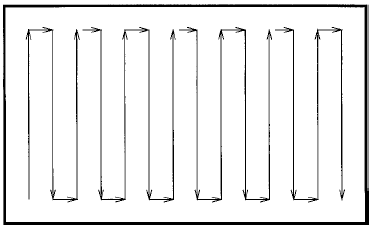
\includegraphics[width=0.45\textwidth]{figs/boustrophedon}
 	\caption[Cobertura pelo método de \textit{boustrophedon}]{Cobertura pelo
 	método de \textit{boustrophedon} \\ Fonte: adaptado de
 	de~\cite{choset2000coverage}}
 	\label{fig::boustrophedon}
\end{figure}

% exact cellular de composition
% Bountrophedon Path
% Coverage path planning
% covering salesman problem
% lawnmower problem

O sistema EMMA de revestimento por aspersão térmica, realiza a tarefa sobre uma
superfície suavemente curva, que representa o perfil hidráulico da pá de uma
turbina Kaplan. Como um dos requisitos do processo é manter a distância fixa
entre a pistola de revestimento e a pá, a trajetória não está restrita a apenas
um plano. \citet{8206216} apresentam uma metodologia que, dado um modelo CAD da
superfície e os parâmetros do processo, realiza-se pelo método RBF
(\textit{radial basis function}) a programação da trajetória para cobrir aquela
superfície. A Figura~\ref{fig::coat_blade} apresenta o modelo CAD da simulação
de revestimento robótico da pá pela metodologia proposta, onde a linha azul
representa o caminho percorrido sobre a superfície.

\begin{figure}[h]
	\centering 
 	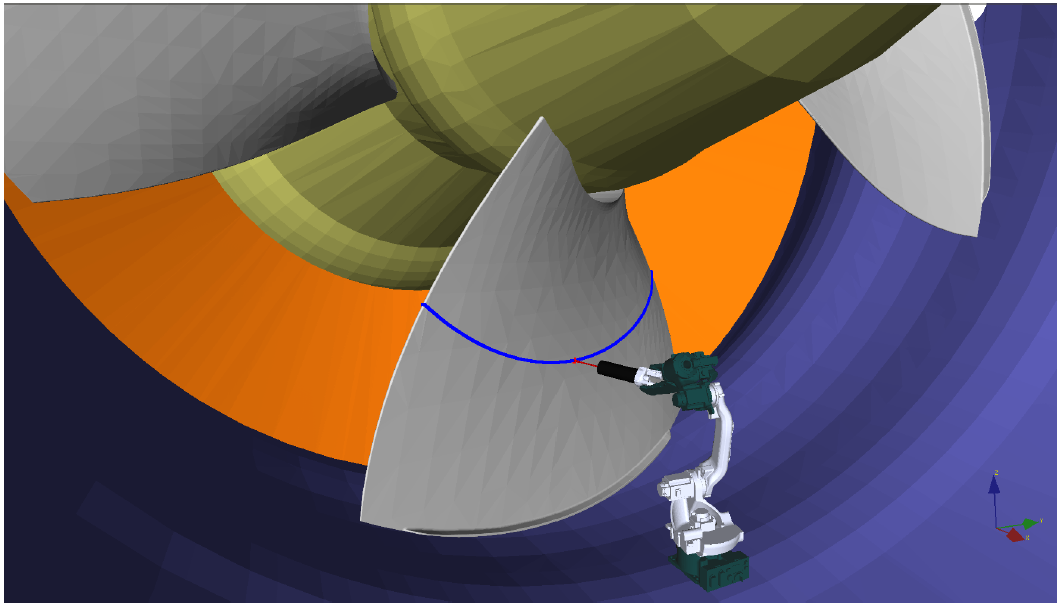
\includegraphics[width=0.75\textwidth]{figs/coat_blade}
 	\caption[Revestimento da face curva de uma pá]{Revestimento da face curva de
 	uma pá. \\Fonte: \citet{8206216}}
 	\label{fig::coat_blade}
\end{figure}

Devido à complexidade deste método, necessidade de ferramentas especiais e por
não acrescentar diferenças significativas esperadas para o resultado da dinâmica
robô-base, é utilizado o método de \textit{boustrophedon} para planejamento do
caminho, considerando os requisitos do processo de revestimento para
planejamento da trajetória.



\subsection{Dinâmica e Equações de Movimento}

O estudo da dinâmica relaciona o movimento de um sistema multicorpos às forças
externas e de inércia que nele atuam. Nesta seção apresenta-se os métodos
clássicos para derivar as equações que regem o movimento do sistema. Outros
métodos também foram explorados historicamente, como as equações de
Hamilton~\cite{shabana2013dynamics},
Boltzmann-Hamel~\cite{papastavridis1994boltzmann} e
Gibbs-Appell~\cite{gibbsappell}, e podem ser encontrados na literatura.
 
\subsubsection{Equações de Newton-Euler}

A formulação de Newton-Euler são uma combinação das Leis de Newton para sistemas
de partículas, e das Leis de Euler, que introduziram os princípios da dinâmica
para corpos rígidos. 

Considerande-se novamente o sistema da Figura~\ref{fig::sist_refs}. Pela segunda
lei de Newton, tem-se que o somatório das forças $F$ que agem sobre o corpo B de
massa $m$ é igual a variação da quantidade de movimento $G$, ou seja:
%
\begin{equation} \label{eq::newton}
	\mathbf{F} = {^R}{\dot{\mathbf{G}}}^{B}
\end{equation}
%
Onde:
%
\begin{equation}
	\mathbf{G}^{B} = m {^R}\dot{\textbf{u}}^{B}
\end{equation}
%


De forma similar, as equações que descrevem a dinâmica do movimento angular são
determinadas, pela equação Euler, como a variação da quantidade de movimento
angular $H$ igual ao somatório dos momentos externos, com respeito
ao centro de massa, que agem sobre o corpo.
%
\begin{equation} \label{eq::euler}
	\mathbf{M} = {^R}{\dot{\mathbf{H}}}^{B}
\end{equation}
%
Tal que a variação da quantidade de movimento angular pode ser escrita como:
%
\begin{equation}
	{^R}{\dot{\mathbf{H}}}^{B} = In_B \cdot {^R}\dot{\boldsymbol{\alpha}}^{B} +
	{^R}\boldsymbol{\omega}^{B} \times In_B \cdot {^R}\boldsymbol{\omega}^{B}
\end{equation}
%
Onde $In_B$ representa o tensor de inércia do corpo B, com respeito ao centro de
massa e alinhado ao sistema de coordenadas local.

As equações~\ref{eq::newton} e \ref{eq::euler} fornecem as 6 equações de
movimento do sistema MBS da Figura~\ref{fig::sist_refs}. Para um caso geral, e
de sistemas de corpos conectados, são formuladas as equações de movimento de
cada corpo, o número de graus de liberdade é reduzido e parte destas 6 equações
de movimento são usadas para determinar as forças e momentos de
contato~\cite{tenenbaum2006fundamentals}.


% The Newton-Euler laws are a combination of the second law of Newton
% (sum of forces equals change of momentum) and Euler's law for the
% change of angular momentum. Both laws lead for an n-body system to a
% set of 6n second-order differential equations describing the dynamic
% behaviour of the system. ``Sol, p.7''

% The dynamics of multibody systems is based on classical mechanics. The most
% simple element of a multibody system is a free particle which can be treated by
% Newton’s equations published in 1686 in his “Philosophiae Naturalis Principia
% Mathematica” [111]. The principal element, the rigid body, was introduced in 1775
% by Euler in his contribution entitled “Nova methodus motum corporum rigidarum
% determinandi” [43]. For the modeling of constraints and joints, Euler already used
% the free body principle resulting in reaction forces. The equations obtained are
% known in multibody dynamics as Newton–Euler equations.  ``Schielen, p.149''

%\subsubsection{Princípio de d'Alembert}

% A system of constrained rigid bodies was considered in 1743 by d’Alembert in his
% “Trait´e de Dynamique” [32] where he distinguished between applied and reaction
% forces. D’Alembert called the reaction forces “lost forces” having the principle
% of virtual work in mind. A mathematical consistent formulation of d’Alembert’s
% principle is due to Lagrange [89] combining d’Alembert’s fundamental idea with
% the principle of virtual work. As a result a minimal set of ordinary
% differential equations (ODE) of second order is found. ``Schielen, p.150''


\subsubsection{Equações de Lagrange}

O método Lagrangeano requer as propriedades de energia do sistema mecânico para
computar as equações de movimento. Esta técnica tem a vantagem de precisar
apenas das energias cinética e potencial do sistema e,
segundo~\citet{murray1994mathematical}, tende a ser menos sujeita a erros do que
somar as forças inerciais, de Coriolis, de atuadores, e outras que atuam nos
elos do robô, por exemplo.

Para escrever as equações de movimento, deve-se definir primeiro o
Lagrangeano, $L$:
%
\begin{equation}
	L(q, \dot{q}) = T(q, \dot{q}) - V(q)
\end{equation}
%
Onde, $T$ é a energia cinética, $V$ a energia potencial do sistema e
$q$ as coordenadas generalizadas.

Então as equações de movimento do sistema, em notação vetorial, podem ser dadas
por:
%
\begin{equation}
	\frac{\mathrm{d} }{\mathrm{d} t}\frac{\partial L}{\partial \mathbf{\dot{q}}} -
	\frac{\partial L}{\partial \mathbf{q}} = \boldsymbol{\Upsilon}
\end{equation}
%
Onde $\boldsymbol{\Upsilon}$ são as forças externas agindo sobre cada
coordenada generalizada do sistema.

O método de Lagrange é interessante sobretudo porque reduz o número de equações
necessárias, de $n$, o número de partículas do sistema, para $m$, o número de
coordenadas generalizadas. Em contrapartida ao método de Newton-Euler, este
não requer a consideração das forças internas ou de restrição do sistema MBS, o
que reduz o número de equações a serem resolvidas.



% A systematic analysis of constrained mechanical systems was established in
% 1788 by Lagrange [89], too. The variational principle applied to the total kinetic
% and potential energy of the system considering its kinematical constraints and the
% corresponding generalized coordinates result in the Lagrangian equations of the
% first and the second kind. Lagrange’s equations of the first kind represent a set of
% differential-algebraical equations (DAE) while the second kind leads to a minimal
% set of ordinary differential equations (ODE). ``Schielen, p.150''

\subsection{Sophia-Maple e Método de Kane}\label{sec::sophia_kane}

Sophia é um conjunto de rotinas implementado para Maple. O programa foi
desenvolvido pelo professor Martin Lesser do KTH Royal Institute of Technology,
Suécia, e sua sintaxe e utilização está bem detalhada no livro intitulado
``\textit{The Analysis of Complex Nonlinear Mechanical
Systems}''\cite{lesser1995analysis}. Sophia foi desenhado especificamente para
modelagem simbólica de sistemas mecânicos multicorpos, e oferece uma forma
sistemática e simples de se chegar às equações de movimento do sistema, através
do método de Kane. Posteriormente foram implementadas por
\citet{lennartsson1999efficient} melhorias no Sophia para eficiência algébrica e
também o pacote \texttt{exmex}, para exportação das equações de movimento para
solução numérica no MATLAB ou Octave.

\subsubsection{Kane}

A formulação de Kane 



Este plano é uma generalização da superfície que restringe o movimento do
sistema MBS e é obtido pela diferenciação das velocidades com respeito
às coordenadas generalizadas, conforme visto na seção~\ref{sec::cinematica}. As
velocidades parciais são calculadas pela expressão das velocidades
generalizadas, na equação~\ref{eq::velgen}. O termo explicitado na
equação~\ref{eq::tau} define o vetor tangente associado a i-ésima coordenada
generalizada.
%
\begin{gather}
%eq1
	^{R}\mathbf{v} = \frac{\mathrm{d} \mathbf{r}}{\mathrm{d} t} = \sum_{i}^{n}
	\dot{q_{i}} \frac{\partial r}{\partial q_{i}} + \frac{\mathrm{d}
	q_{i}}{\mathrm{d} t} \label{eq::velgen}\\
%eq2
	\dot{q_{i}} \frac{\partial r}{\partial q_{i}} = \tau_{i} \label{eq::tau}
\end{gather}
%

\subsubsection{Notação de Lesser e Lennartsson}


% -.~.-.~.-.~.-.~.-.~.-.~.-.~.-.~.-.~.-.~.-.~.-
\section{Análise dinâmica de estruturas}

\subsection{Matriz de rigidez} \label{sec::rigidez}

\subsection{Amortecimento proporcional} \label{sec::amortecimento}

\subsection{Frequência Natural, Modo de Vibração e Amortecimento}
\label{sec::param_mod}

\subsection{Ensaio experimental de vibrações}


% -.~.-.~.-.~.-.~.-.~.-.~.-.~.-.~.-.~.-.~.-.~.-
\section{Manipuladores robóticos industriais}\label{sec::manind}

\subsection{Manipuladores flexíveis}

\subsection{Manipuladores sobre bases flexíveis}

\subsection{Tarefas de precisão utilizando manipuladores robóticos}

\subsection{Sistema de revestimento por asperção térmica} \label{sec::hvof}

\subsection{Tarefas robóticas \textit{in-situ}} \label{sec::insitu}



\begin{figure}[h]
	\centering 
 	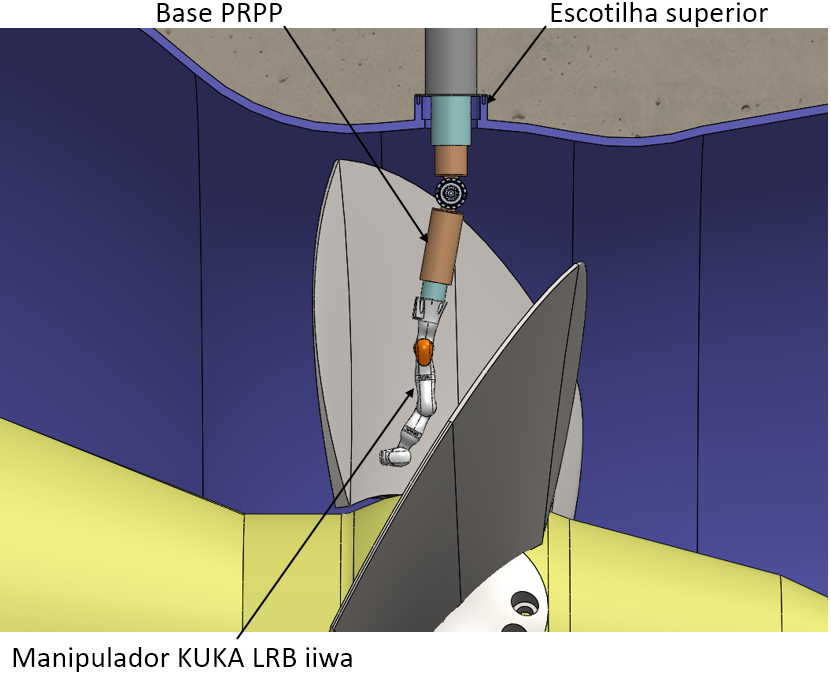
\includegraphics[width=0.85\textwidth]{figs/base_telesc_turbina}
 	\caption{Base telescópica PRPP para manutenção de revestimento
 	\textit{in-situ}}
 	\label{fig::base_telesc_turbina}
\end{figure}

\begin{figure}[h]
	\centering 
 	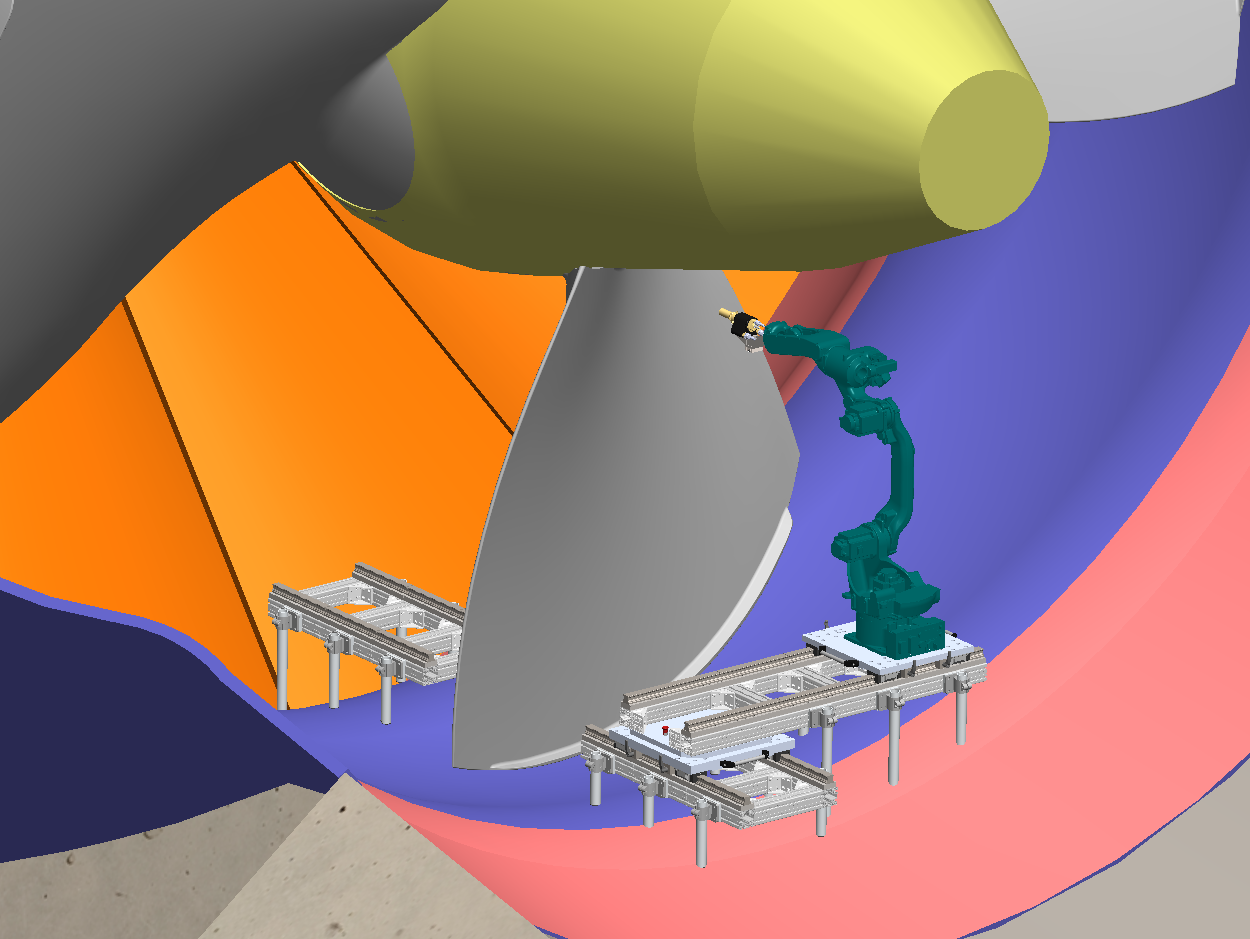
\includegraphics[width=0.85\textwidth]{figs/prp_turbina}
 	\caption{Base modular PRP para manutenção de revestimento \textit{in-situ}}
 	\label{fig::prp_turbina}
\end{figure}




















